\documentclass[11pt]{article}
\usepackage[nohead,margin=2cm,includefoot]{geometry}
\geometry{verbose,letterpaper,tmargin=1in,bmargin=1in,lmargin=1in,rmargin=1in}
\renewcommand{\familydefault}{\sfdefault}
\usepackage{graphicx}
\usepackage{hyperref}
\usepackage{listings}
\title{PIBASE user guide. ver 2010\\
\includegraphics[scale=0.5]{pibase_blue_web.pdf}}
\author{Fred P. Davis, HHMI-JFRC\\{\tt davisf@janelia.hhmi.org}\\\url{http://pibase.janelia.org}}
\begin{document}

\maketitle

\begin{abstract}
This document describes how to use PIBASE through the (1) web, (2) mysql, and (3) perl api interface.
\end{abstract}

\section{Introduction}
PIBASE is a collection of protein structural domain interfaces extracted from the \href{http://www.rcsb.org/pdb}{Protein Data Bank} and \href{http://www.ebi.ac.uk/msd-srv/prot_int/pistart.html}{PISA} structure databases using \href{http://scop.mrc-lmb.cam.ac.uk/scop/}{SCOP} and \href{http://www.biochem.ucl.ac.uk/bsm/cath/}{CATH} domain definitions. It was designed to provide answers to questions regarding the structures and organization of protein complexes and the interfaces within. It also  provides a unified way of accessing domain properties, such as boundary definitions, surface areas, secondary structure assignemnts, {\it etc}, in a SQL-queryable fashion.

This document gives examples of how to query PIBASE through the web, MySQL, and Perl interfaces.

\begin{figure}
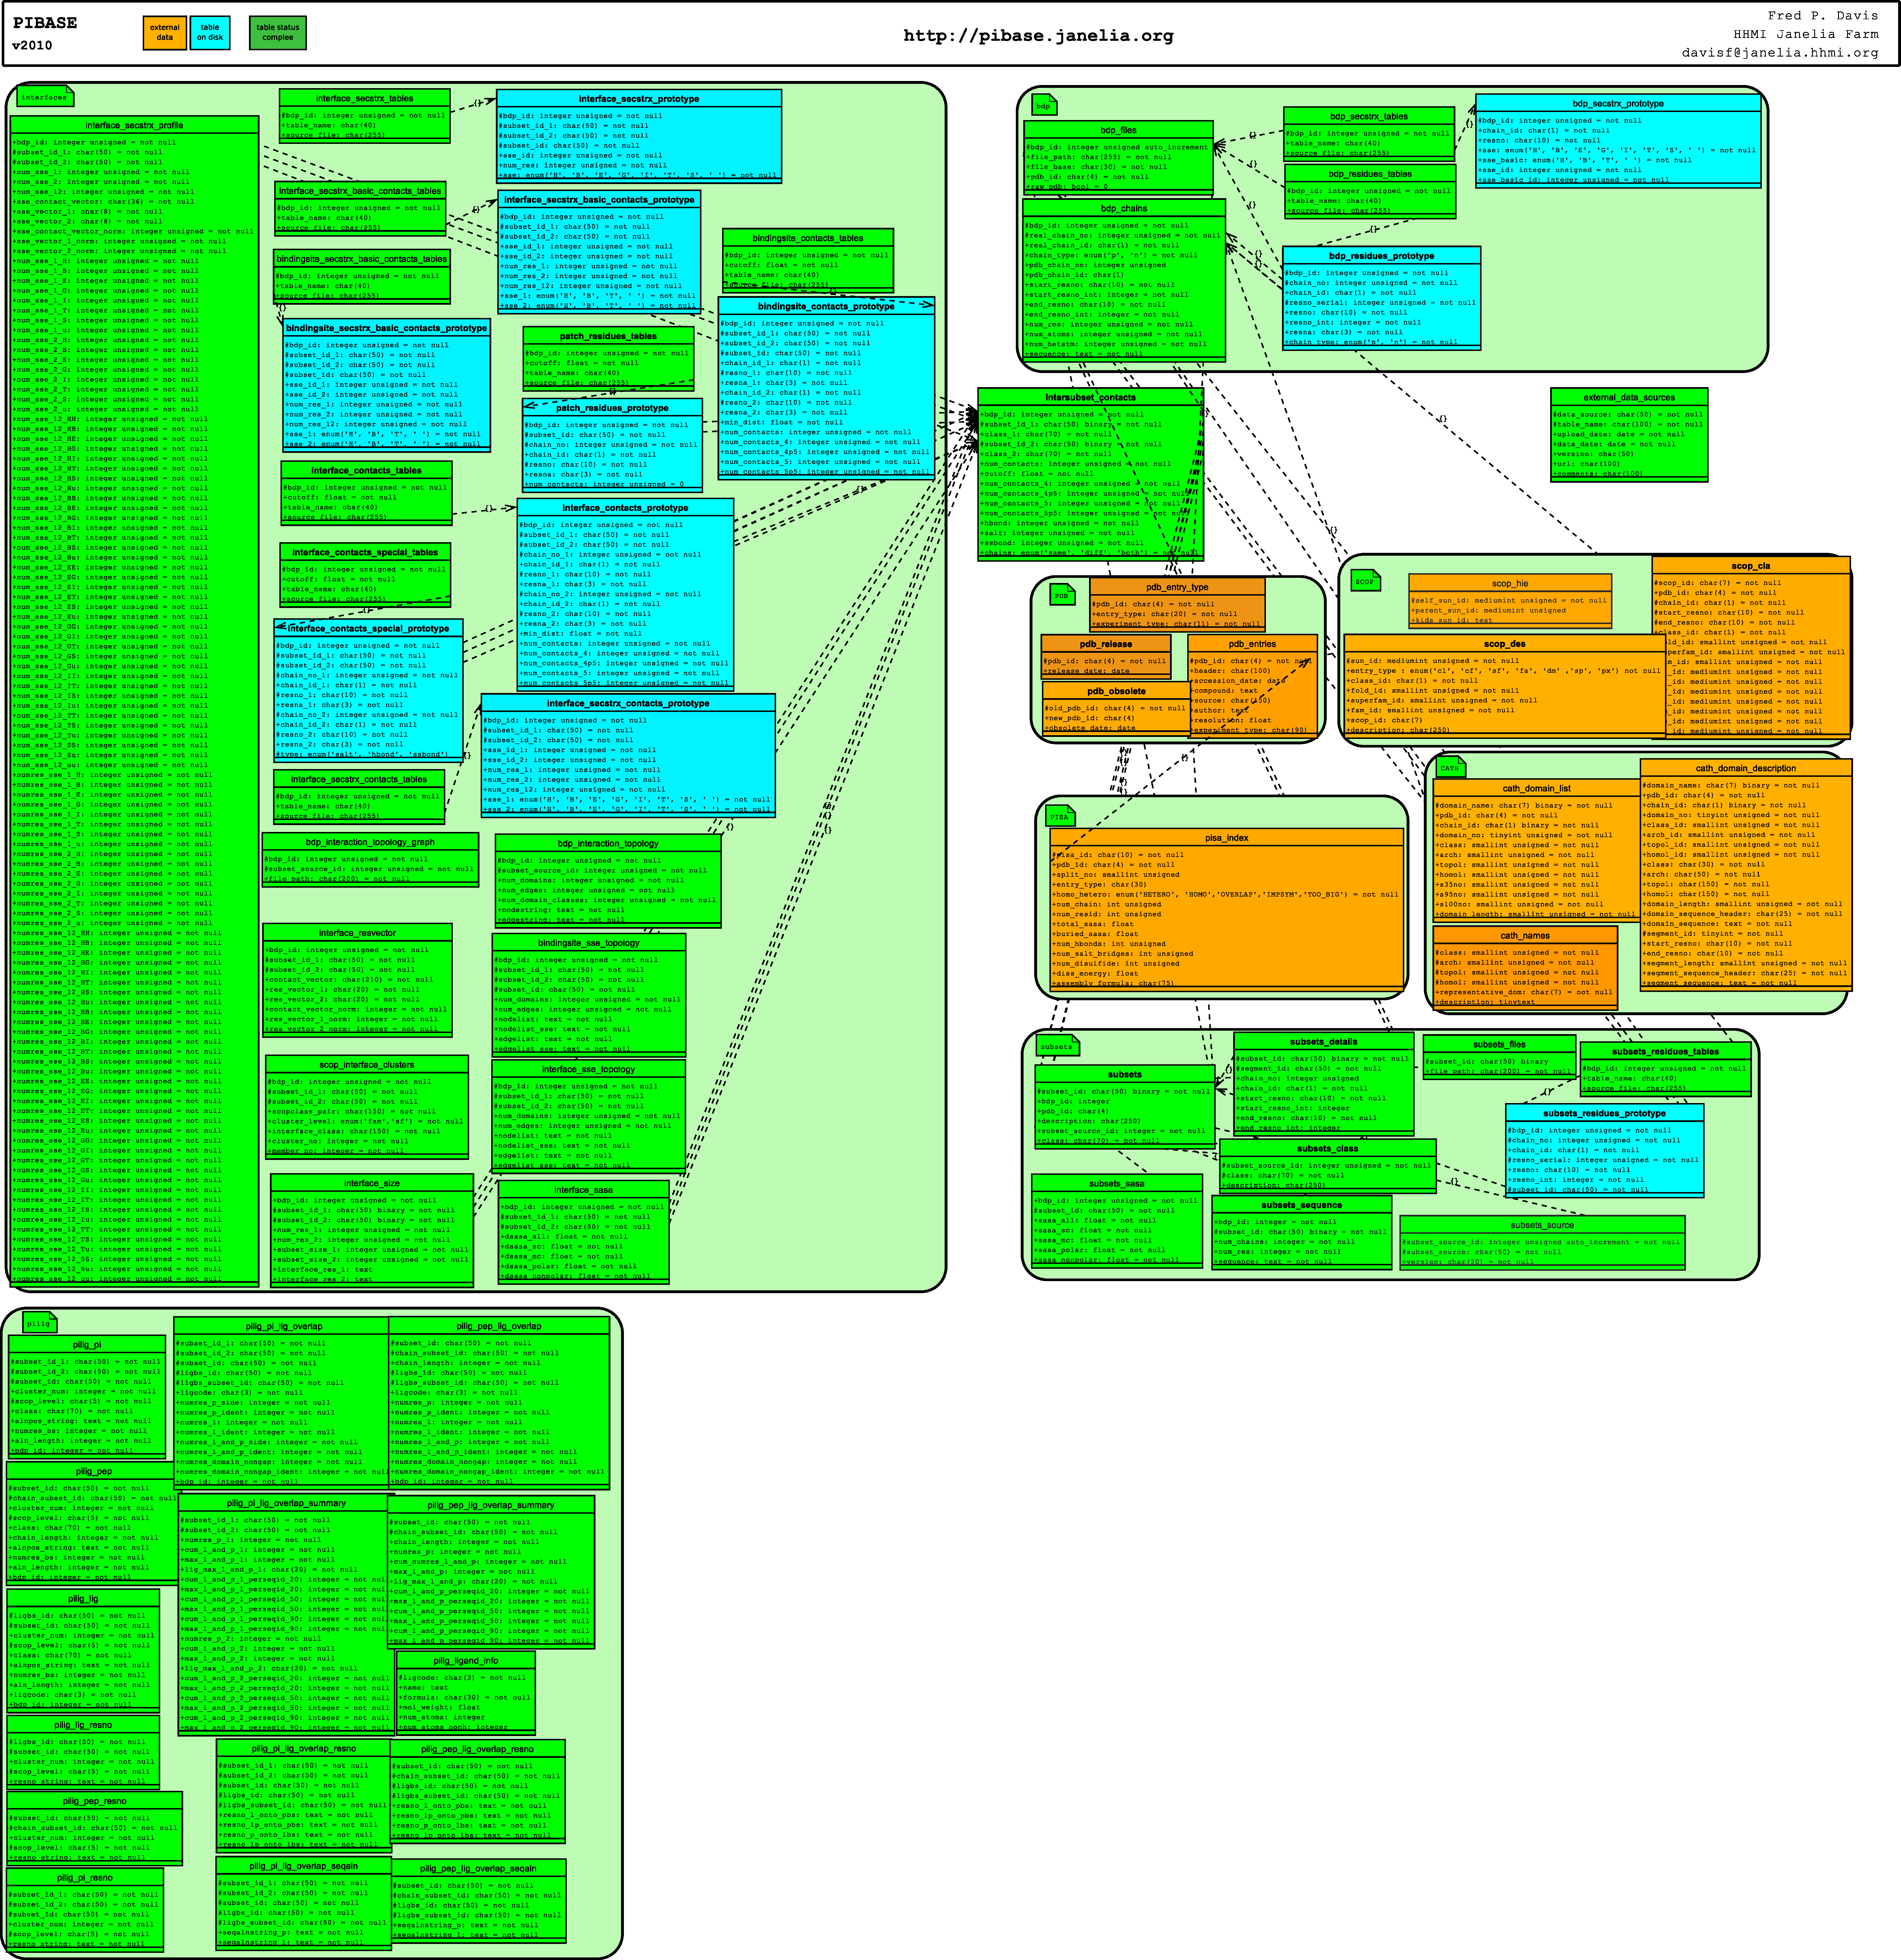
\includegraphics[scale=0.125,angle=90]{design/PIBASE_schema.pdf}
\caption{PIBASE database schema.}
\end{figure}

\section{Using PIBASE}

\subsection{web interface}

\subsection{MySQL interface}

\subsection{Perl interface}

\end{document}
